\chapter{Umsetzung}\label{chap:Umsetzung}

\chapterstart

Folgend wird die Umsetzung beschrieben, die in mehrere Bereiche aufgeteilt wurde. Diese Teilbereiche gliedern sich wie folgt:
\begin{itemize}
	\item Vorbereitung der Entwicklungsumgebung
	\item Erstellen des Reverenzservers in Javascript mit Node.js
	\item Erstellen des Testservers in Swift mit Perfect
	\item Vergleich der beiden Server
	\item Fazit
\end{itemize}

\section{Die Umgebung}
\label{sec:dieumgebung}

Für die Entwicklung des Swift-Servers musste eine Linux Distribution gefunden werden, die den Ansprüchen einer Entwicklungsumgebung entspricht. Mehrere Faktoren spielten dabei eine Rolle. Die wichtigsten Punkte dabei waren die Stabilität der Distribution, die Möglichkeit Entwicklungsumgebungen beziehungsweise Programme zu installieren ohne großen Aufwand mit dem auflösen von Abhängigkeiten zu haben, und geringer Wahrscheinlichkeit möglicher Inkompatibilität. Weiters sollte es möglich sein diese als Virtuelle Maschine laufen zu lassen. 

\paragraph{Stabilität}
Die Stabilität ist wichtig da Swift die Sprache "C" verwendet und es die Möglichkeit gibt, die Virtuelle Maschine, zum Beispiel durch das Abstürzen des OS zu beschädigen. Außerdem sollte es möglich sein, Programme aller Art auf dem OS zu installieren, sodass es keine Überraschungen im Laufe des Projektes gibt. Weiter wurde auch seitens der Swift-Entwickler Ubuntu empfohlen. Daher fiel die Wahl auf die zu diesem Zeitpunkt aktuelle Ubuntu Version 16.04 LTS, da diese auch möglichst leichtgewichtig ist. 

\paragraph{Entwicklungsumgebung}
Da Swift eine noch nicht sehr weit verbreitete Sprache außerhalb der Mac-Welt ist, war es eine Herausforderung einen IDE, die auf Linux lauffähig ist, zu finden, in der eine Unterstützung in Form von zum Beispiel Syntaxhighliting oder Autovervollständigung für Swift zur Verfügung steht. Zur Lösung des Problems wurde \textit{CLION} von \textit{JetBrains} \parencite{jetbrain} in der Version 2017.2 verwendet, das ein Plugin für Swift bereithält.

\paragraph{Virtuelle Maschine}
Für das Betriebssystem musste die Möglichkeit bestehen, es als eine Virtuelle Maschine auf einem PC lauffähig zu bekommen. Dazu wurde als Umgebung für die VM \textit{VirtualBox} von \textit{Oracle} installiert und darauf die vorhin erwähnte Ubuntu 16.04 LTS Distribution aufgesetzt.

\section{Der Reverenz-Server}
\label{sec:derreverenzserver}

Um den Swift-Server vergleichen zu können, wurde zuvor ein Server benötigt, der verschieden serverseitige Anforderungen erfüllt. Anforderungen, die nicht direkt mit Node.js und Express.js in Verbindung stehen, zum Beispiel Responsive Web, welches mit CSS erreicht wurde, werden hier nicht berücksichtigt. Dieser Server wurde bereits im Zuge der Lehrveranstaltung "Rich Internet Application" von Michael Rotinger, Stefan Moder und Christian Hofer implementiert und erfüllt folgende serverseitige Anforderungen: 
\begin{itemize}
	\item Verwendung eines aktuellen Frameworks
	\item Dynamische Website Erstellung
	\item Registrierung, Speichern von Userdaten und verschlüsseln des Passwortes
	\item Login und Sessionverwaltung
	\item Caching
	\item Socketverbindung
	\item Model View Controller Pattern
	\item Logging
	\item Kompression
\end{itemize}

\paragraph{Framework}
Der Server ist in JavaScript geschrieben, wobei hier Node.js mit dem Framework Express verwendet wurde. Node.js ist eine I/O-Umgebung, die als einziger Thread auf dem Server läuft, der niemals geblockt wird. Stattdesen arbeitet es auf Event-Basis mit Callbacks. Jeder Request ist als Event zu verstehen und wird zum Beispiel als Datenbankabfrage erkannt. Der Mainthread wartet dabei nicht darauf, dass die Datenbankabfrage fertig ist und blockiert inzwischen, sondern kann in der Zwischenzeit weitere Requests behandeln. Bei Beendigung des I/O-Prozesses wird durch den Callback die eventuelle Response gesendet. Neben der Asynchronität von Node.js ist die Geschwindigkeit von dieser JavaScript-Maschine enorm. Entwickelt wurde Node.js auf Basis der "Google Chrome V8 engine" die JavaScipt enorm schnell bearbeiten kann. Unterstützt durch das Framework Express können weitere Vorteile wie Middleware und modulbasierte Plugins verwendet werden. Weitere Vorteile von Express sind, dass es ein offenes, schnelles und unkompliziertes Web-Framework ist, das auch mobile Anwendungen unterstützt. Grundsätzlich werden 4 Hauptaufgaben von Express.js zur Verfügung gestellt:
\begin{itemize}
	\item Middleware: diese bildet ein Array mit Funktionen, mit denen Request standardmäßig vorbearbeitet werden können, zum Beispiel setzen einer Variabel
	\item Routing: ist ein fester Bestandteil des Frameworks und ist mit dem Unterschied, das es aufgerufen werden muss mit einer Middleware vergleichbar
	\item Erweiterungen für Request und Response Objekte
	\item Views: Dynamisches rendern von HTML
\end {itemize} 
Diese vier Bestandteile ermöglichen ein schnelles Erstellen eines WebServices \parencite{expressinaction}. 
Express wird von der Stiftung Node.js projektiert und verwaltet und wird auch ständig weiterentwickelt \parencite{expressjs}. Mittlerweile steht auch auf Basis von Express.js ein neues Framework LoopBack zur Verfügung, welches die Entwicklung von dynamischen end-to-end REST APIs für verschiedene Geräte und Browser zulässt, inklusive der Entwicklung von Client Application auf Android, iOS und AngularJS SDKs \parencite{loopback}.

\paragraph{Dynamische Websites}
Die Websites können mit der Eingabe von Usern verändert werden, zum Beispiel durch die Anzeige des Usernamens auf der Website. Dies soll serverseitig ermöglicht werden bevor das HTML an den Client gesendet wird. Im Reverenzserver übernimmt dies das Modul "Handlbars". Diese Module ermöglichen es HTML-Skelete zu erstellen und mit Eingaben zu befüllen.

\paragraph{Registrieren, speichern, verschlüsseln}
Der Server ermöglicht es dem Client sich in einen gesicherten Bereich zu bewegen, dazu erfolgt zuvor eine Registrierung. Dazu werden die Daten des Users in Form eines JSON-Strings im Filesystem gespeichert. Für das Filehandling wurde das standardmäßig in Node.js enthaltene Modul "fs" verwendet. Dieses Modul übernimmt jegliche I/O-Aufgaben betreffend dem Filehandling, wie auch das Einlesen von Dateien. Eine Variation wäre das Verwenden einer Datenbank zum Beispiel Redis. Bevor das Passwort des Users gespeichert wird, soll dieses natürlich verschlüsselt werden, welches mit dem Modul "bcrypt-nodejs" erreicht wurde. Dieser verwendet eine "salted" SHA256 Verschlüsselung, welches asynchron oder synchron ausgeführt werden kann. 

\paragraph{Login und Session}
Nach dem Einloggen des Users wird auf dem Server eine explizite Session gestartet. Diese wird automatisch durch Express und dem Modul "express-session" verwaltet und benötigt nur die Initialisierung und die Löschung der Session. Dadurch ist eine minimale Sessionverwaltung erreicht.

\paragraph{Caching}
Das Caching wurde durch das Setzen von Caching Headern erreicht. Das Setzen dieser Header wurde durch Aufruf von selbst implementierten Methoden erreicht, welche wiederum im Laufe der Requestbehandlung aufgerufen werden. Dazu wurde kein externes Modul verwendet beziehungsweise benötigt.

\paragraph{Socketverbindung}
Für die Socketverbindung im Server, um einen Chat zu betreiben, wurde das Modul "socket.io" verwendet. Dieses Modul bildet einen Adapter, um eine unkomplizierte Errichtung einer WebSocket-Verbindung zu implementieren.

\paragraph{Model View Controller Pattern}
Der Reverenzserver wurde im MVC-Pattern geschrieben, da diese zu den wichtigsten Design Patterns in der Webentwicklung zählt. Das MVC ist eines der offensten Patterns und behält sich einen großen Spielraum bereit. Das Pattern kann mehr als allgemeine Empfehlung gesehen werden als eine Anleitung, da es dem Entwickler selbst obliegt, zu entscheiden, welche Klassen, Objekte, Methoden oder Funktionen zu den einzelnen Fraktionen des MVC gehören. Beim Implementieren des Servers wurde eine grobe Einteilung getroffen. Controller nehmen Request entgegen, steuern den Kontrollfluss und senden die Response, Models führen Operationen auf Daten aus und Views sind für die Generierung des HTML-Codes zuständig.

\paragraph{Logging}
Für eine Erleichterung der Entwicklung und im späteren Betrieb wurde auch eine Logging miteingerichtet, welches mit verschiedenen Logging-Level arbeitet. Die Informationen werden nicht nur auf der Konsole ausgegeben, sondern auch in ein Log-File geschrieben und wird für eventuelle Debugging auch im File System gespeichert.

\paragraph{Kompression}
Die HTML Daten werden vor der Übermittlung an den Client per gzip komprimiert. Dafür wurde das Modul \textit{compression} verwendet.

\section{Der Swift-Server}
\label{sec:derswiftserver}
Um einen Server in Swift zu programmieren, muss die in \ref{sec:dieumgebung} erwähnte Ubuntu Distribution mehrere Vorraussetzungen erfüllen. Verschiedene C-Bibliotheken und "Clang" müssen installiert werden. Diese einzelnen Bedingungen und deren Installationsbedingungen und -vorgänge werden nun näher erläutert.

\subsection{Swift auf Linux installieren}
Für die Installation von Swift sind vier wichtige Bibliotheken bzw. Programme notwendig, die vorinstalliert werden müssen, damit die danach installierte Swift-Toolchain installiert und ausgeführt werden kann. 
\begin{itemize}
	\item clang
	\item libicu-dev
	\item libcurllpp
	\item git (optional)
\end{itemize}

\paragraph{Clang}
\label{para:clang}
Clang ist ein Front-End Compiler für C-basierte Sprachen wie C, C++, Objective C/C++, OpenCL C und andere Sprachen für den LLVM Compiler. Einige Ziele des Clang sind ein schnelles compilieren mit wenig Speicherverwendung zu erreichen, ausführliche Diagnose- und Fehlerberichte zu erstellen und auszugeben und GCC kompatibl zu sein. Dadurch wird eine bessere Kompatibilität mit verschiedenen IDEs erreicht und Sprachen wie Swift können auf Betriebssystemen kompiliert werden. Clang ist unter der BSD Lizenz verfügbar und darf daher auch als integraler Bestandteil von kommerziellen Projekten verwendet werden \parencite{clang}. Clang ist bei der Kompilierung von Code bis zu drei mal so schnell als zum Beispiel der GCC. Zusätzlich hält der Clang Compiler auch den Clang Static Analyzer bereit, der automatisch Bugs im Code \parencite{llvm}. Im Projekt ist Clang nur bei der Compilierung beteiligt und wird im Code nur einmal direkt verwendet. 

\lstset{caption=OS Prüfung, basicstyle=\small\ttfamily, label=lst:osprüfung, language=C}
\begin{lstlisting}
// Save guard against ios or windows usage
#if !os(Linux)
import Glibc
print("We are sorry this is only meant to be run on Linux")
exit(1)
#endif
\end{lstlisting}

Bei diesem Codeteil handelt es sich um eine Prüfung des Betriebssystems, wobei darauf geprüft wird, dass das System eine Linux Distribution ist und ansonsten abgebrochen wird. Die Syntax dieser OS Prüfung entspricht Clang und wird daher auch direkt von dieser kompiliert. Das compilieren von Swift wird ebenfalls von Clang übernommen, welches zu Maschinencode für die LLVM überführt wird und auf der Objctive-C runtime läuft.

\subparagraph{Der LLVM Compiler}
Ein Fehler wäre zu denken, LLVM wäre ein Acronym, tatsächlich ist es der vollständige Name des Compilers. Das LLVM begann als Wissenschaftsprojekt auf der Universiät von Illinoi und hat das Ziel, eine moderne SSA-basierte Kompilierungsstrategie zur Verfügung zu stellen. Dabei soll es möglich sein, statische wie auch dynamische Kompilierung von verschiedenen Programmiersprachen durchzuführen. LLVM ist derzeit zu einer großen Sammlung von modularen und wiederverwendbaren Compilern und Toolchains geworden, die unter der BSD Lizenz verfügbar sind \parencite{llvm}. Tatsächlich arbeitet der LLVM Compiler mit einer Vielzahl von compiler Techniken. Darüber hinaus verfügt er über eine Codeoptimierung und Generierung, den llvm-gcc als Backend und den Clang Front-end und unterstützt die Microsoft Intermediate Language und die .Net Vitual Machine. Der LLVM wurde entwickelt, weil ältere bereits existierende C Compiler nicht mehr weiterentwickelt wurden. Die größte Stärke des LLVM liegt darin, dass er aus mehreren Compiler-Modulen besteht, die sich gegenseitg ergänzen. Daraus wurden wiederum Compiler gebaut, die für verschiedene Aufgaben geeignet sind z.B. als erweiterter C-Compiler oder als spezialisierte Runtime-Maschine. Ein weiterer Vorteil ist das der llvm-gcc 4.2 mit den gcc command line Optionen und Sprachen, sowie dem makefiles kompatibel ist \parencite{llvmpulbic}.

\paragraph{libicu-dev und libcurllpp}
Diese Pakete sind Bibliotheken, die benötigt werden, um die Ausführung aller Swift-Bibliotheksfunktionen auszuführen. Nähere Informationen zu diese Paketen sind für das Projekt nicht notwendig.

\paragraph{Git}
Für die Versionierung und der gemeinsamen Bearbeitung wurde Git verwendet, das jedoch nicht direkt für den Server notwendig ist und soll daher nur erwähnt bleiben.

\paragraph{Installation}
Zur Installation wird der aktuelle Release heruntergeladen. Diese liegt als .tar.gz vor und kann in ein beliebiges Verzeichnis entpackt werden. Als Erleichterung wurde der Pfad in die Umgebungsvariable von Ubuntu hinzugefügt, um ein leichteres compilieren möglich zu machen bzw das Ausführen der REPL zu erleichtern. Der Server wurde mit dem Release 3.1.1 für Ubuntu 16.10 entwickelt.

\subsection{Das Swift Package}
\label{sec: dasswiftpackage}
Die Swift Sprache ist als Sammlung verschiedener Projekte gegliedert:
\begin{itemize}
\item Swift Compiler
\item Standard Bibliothek 
\item Core Bibliothek
\item LLDB Debugger
\item Swift Package Manager
\item Xcode Playground support
\end{itemize}

\paragraph{Swift Compiler}
Der Swift Compiler übersetzt den Source Code in effiziente und ausführbare Maschinensprache. Zuerst erfolgt das Parsen des Codes und das Erstellen des Abstract Syntax Trees, der für die darauffolgende semantische Analyse benötigt wird. Aus dem AST wird somit ein "well-formed, fully-type-checked" AST. Die semantische Analyse stellt sicher, dass es möglich ist zu compilieren.  Danach wird der Clang Importer benötigt, der verschiedene Clang Module importiert, die benötigt werden, um den AST auf C oder Objective-C APIs umzusetzen. Als nächster Schritt wird der AST mithilfe der Swift Intermediate Language optimiert und in eine sogenannte "raw" SIL umgeformt. Aus der SIL wird wiederum die "canonical" SIL erstellt. Dies wird erreicht, indem eine weitere sogenannte garantierte Transformation durchgeführt wird, in der zusätzliche Datenflussdiagnostik durchgeführt wird, zum Beispiel die Verwendung von nicht initialisierten Variablen. Danach wird nochmals eine Optimierung über die SIL durchgeführt wie das automatische Referenzieren, zähl-Optimierung, Devirtualisierung und allgemeine Spezialisierung. Ab diese Punkt wird der Code weitergegeben an die LLVM IR Code Generierung, sodass aus der SIL eine LLVM IR wird und diese durch die LLVM zu Maschinen Code übersetzt werden kann \parencite{swiftcompiler}. 

\paragraph{Standard Bibliothek}
\label{para:standardbibliothek}
Die Standard Bibliothek von Swift hält verschiedene Beschreibung von Daten-Typen, Protokollen und Funktionen bereit. Auch primitive Typen werden hier beschrieben. Die Standard Bibliothek wird in drei Teile gegliedert:
\begin{itemize}
\item core: Darin befinden sich alle Definition für Daten-Typen, Protokolle und Funktionen
\item runtime: Dies wird als Zwischenschicht zwischen Compiler und der Core Standard Bibliothek geführt. Diese ist für dynamische Operationen zuständig wie z.B. das Casten oder Memory Management
\item SDK Overlays: Hält verschiedene Pakete und Modifikationen bereit, um existierende Objective-C Frameworks in Swift einzubinden
\end{itemize}

Die Standard Bibliothek ist zwar in Swift geschrieben, jedoch weicht sie vom üblichen Swift Code ab. Diese Unterschiede sind auf den Nutzen der Bibliothek zurückzuführen, da diese z.B. benötigt wird, um die SIL zu erstellen oder gesamt als "public" zur Verfügung stehen soll. Zusätzliche Tools wie "gyb" sind notwendig, um sized Integer Typen zu deklarieren oder das Testen ist eng mit dem Compiler verbunden beziehungsweise ohne diesen nicht möglich \parencite{swiftbibliothek}.

\paragraph{Core Bibliothek}
Diese hält verschiedene higher-level Funktionalität bereit als die Standard Bibliothek. Der Hauptteil der Bibliothek wird mit \textit{import Foundation} im Code importiert und damit in einer spezifischen .swift-Datei zur Verfügung gestellt. Erst mit diesem Import steht sie beim compilieren zur Verfügung. Die Bibliothek soll verschiedene stabile und nützliche Features in folgenden Bereichen bereithalten:
\begin{itemize}
\item generell verwendete Typen z.B. URLs, Character Sets, Collections usw. 
\item durchführen von Unit Tests
\item Networking Grundlagen
\item Persistence, Listen, Archive, JSON parsing, XML parsing
\item Datum-, Zeit- und Kalenderfunktionalität
\item OS-Spezifisches Verhalten
\item Interaktionen mit dem File System
\end{itemize}

Diese Bibliothek ist laut Swift.org noch nicht vollkommen und ausreichend entwickelt, sondern ist derzeit im Anfangsstadium. Diese wurde veröffentlicht, um es der Community zu ermöglichen von Anfang an bei der Entwicklung mit zu gestalten und mit zu wirken.  Derzeit sind drei Teile der Bibliothek vorhanden. Diese sind \textit{Foundation}, welche die Basis für alle Swift Projekte darstellt, \textit{libdispatch}, die das Multithreading und Multitasking ermöglicht, sowie \textit{XCTest}, welches ein Framework für das Erstellen von Unit Test bildet \parencite{swiftcore}.

\paragraph{LLDB Debugger}
Der LLDB Debugger ist ein Teil des Clang-Projektes. Besonderheit hier ist, das der Debugger als Grundlage für den Swift REPL dient. Laut Swift.org hat dies folgende Vorteile.
\begin{compactenum}[a)]
\item Der Hauptvorteil ist, dass die REPL einen vollwertigen Debugger zur Verfügung hat, der sogar Breakpoint zulässt.
\item Weiter kann sich die REPL von einem kritischen Error erholen, sodass eine Fehlermeldung angezeigt wird und die REPL nicht neu gestartet werden muss
\item Die REPL erhält Zugang zu jeglichen Sprachfeatures
\item konsistentes Format des Ergebnisses
\end{compactenum}

Diese Vorteile wurden nicht im Zuge der Umsetzung geprüft und sind daher nur ein Übertrag der von Swift.org genannten Vorteile \parencite{swiftdebugger}.

\paragraph{Swift Package Manager}
Swift gliedert sich wie Node.js und Express.js in Modulen. Diese werden wie bei Node.js in einer Package Datei verwaltet. Diese Package.swift Datei enthält alle Abhängigkeiten, die für ein Projekt notwendig sind. Der Eintrag der Abhängigkeit wird manuell durchgeführt, indem diese in die Package.swift eingetragen wird. Diese wird als Array beschrieben und enthält die Source URL und die Version, die heruntergeladen werden soll. Diese Packages könnten danach mit dem \textit{import ...} im Projekt zur Verfügung gestellt werden.
Der Manager erstellt vorab eine Struktur für das Projekt, die aus der \textit{Package.swift} Datei besteht, dem Verzeichnis \textit{Sources} inklusive der Datei \textit{Hello.swift} und einem Testverzeichnis indem bereits die Datei \textit{HelloTests.swift} und \textit{LinuxMain.swift} enhalten sind. Die LinuxMain.swift Datei importiert die notwendige Bibliothek XCTest, welche bereits im Absatz \ref{para:standardbibliothek} beschrieben wurde \parencite{swiftpm}.

\paragraph{Xcode Playground support}
Xcode ist nur in geringen Teilen für Linux von Interesse, da die Hauptfunktionen nur mit der IDE Xcode verwendet werden können. Xcode ist wiederum nur für Mac konzipiert, sodass hierauf nicht näher eingegangen wird.


\section{Vergleich der Implementierungen}

In diesem Kapitel geht es um die Umsetzung des in ref{sec:derreverenzserver} beschriebenen Express.js Servers als Swift-Server. Dieser soll die gleichen Anforderungen erfüllen, welche waren:
\begin{inparaenum}
	\item Verwendung eines aktuellen Frameworks
	\item Dynamische Website Erstellung
	\item Registrierung, Speichern von Userdaten und verschlüsseln des Passwortes
	\item Login und Sessionverwaltung
	\item Caching
	\item Socketverbindung
	\item Model View Controller Pattern
	\item Logging
	\item Kompression.
\end{inparaenum}

\subsection{Framework}
Als Framework für den Swift Server standen zwei verschiedene Frameworks zur Auswahl: 
\begin{itemize}
	\item Perfect: als Toolkit für Anwendungen und REST-Services
	\item Kitura: ein neues WebFramework von IBM
\end{itemize}
An dieser Stelle ist zu erwähnen, dass es ein weiteres Framework namens \textit{Vapor} gibt, welches erst nach der Entwicklung des Servers mit Perfect zu spät entdeckt wurde.

\paragraph{Perfect}
Perfect wird auf deren Homepage als WebServer und Toolkit für Swift-Entwickler beschrieben, um Applikationen und andere REST-Services zu entwickeln. Es kann verwendet werden um clientseitig wie auch serverseitig zu programmieren und wird als ideales Backbone für Cloud und mobile Technologien bezeichnet. Entwickler können damit produktiver arbeiten und benötigen dazu nur eine Sprache. Bereits auf der Homepage wird Perfect mit Node.js selbst verglichen und bietet eine Vielzahl an Bibliotheken an. Diese sollten mit den Node.js und Express.js Modulen, sofern diese benötigt wurden, im Zweck vergleichbar sein, welches in der folgenden Tabelle veranschaulicht wird.

\begin{table}[]
\begin{center}
\begin{tabular}{p{5cm}p{3.5cm}p{4.5cm}}
\rowcolor{gray20}	\textbf{Anforderung}									& \textbf{Node.js}	  		& \textbf{Perfect}								\\ 
\rowcolor{gray5}		Dynamische Website Erstellung							& handlebars					& Workaround								\\ 
\rowcolor{gray20}	Registrierung											& -							& -											\\ 
\rowcolor{gray5}		Filehandling (speichern)								& fs							& Foundation									\\ 
\rowcolor{gray20}	Verschlüsselung										& bcrypt						& SwiftyBeaver								\\ 
\rowcolor{gray5}		Login												& -							& -											\\
\rowcolor{gray20}	Sessionverwaltung									& express-session				& PerfectSession								\\ 
\rowcolor{gray5}		Caching												& - 							& - 											\\ 
\rowcolor{gray20}	Socketverbindung										& socket.io					& PerfectWebSockets							\\ 
\rowcolor{gray5}		Logging												& winston					& PerfectLogger und PerfectRequestLogger		\\ 
\rowcolor{gray20}	Kompression											& compression				& GzipSwift								\\ 
\rowcolor{gray5}		Routing (parsen von Requests und Responses)			& express					& PerfectHTTP								\\
\end{tabular}
\caption{Module der Server} \label{tab:modulederserver}
\end{center}
\end{table}

\subsection{Dynamische Website Erstellung}
Wie der Tabelle zu entnehmen ist, wurde für die dynamische Website-Gestaltung ein Workaround implementiert. Ausschlaggebend dafür war das Fehlen von Kontrollstrukturen beim von Perfect entwickelten Package \textbf{Mustache}. Dieses Package hält wie auch  Handlebars die Möglichkeit bereit, Bereiche eines HTML-Layout bzw. Templates, die mit "\{\{\}\}" gekennzeichnet wurden, mit Variablen zu füllen. Unterschied liegt darin, dass Mustache keine Kontrollfluss-Befehle unterstützt wie z.B. Handlebars mit einer If-Abfrage. 

\lstset{
	caption=Handlebars,
	label=lst:handlebars,
	language=JavaScript,
	basicstyle=\footnotesize\ttfamily,
	tabsize=2,
	showtabs=false,
	keywordstyle=\color{orange}\bfseries,
	commentstyle=\color{darkgray}\ttfamily,
	stringstyle=\color{darkgreen}\ttfamily,
	ndkeywordstyle=\color{blue}\bfseries,
	identifierstyle=\color{black},
}

\begin{lstlisting}
const hbs = require('handlebars');
const layout = require('./layout');
const fs = require('fs');
const logger = require('../controllers/logging.controller').logger;

hbs.registerPartial('chat', fs.readFileSync('./views/partials/Chat.html', 'utf-8'));

function renderChatView(user) {
    logger.debug("renderChatView for: " + user);
    const viewModel = {bodyPartial: 'chat', user: user};
    return layout(viewModel);
}

module.exports = {
    renderChat: renderChatView
};
\end{lstlisting}

Wie im Listing \ref{lst:handlebars} zu sehen ist, wird Handlebars import und in Zeile 10 das zuvor registriert HTML Partial abgerufen und in der Variable viewModel gespeichert. Für das Partial interessant ist, dass es eine Kontrollstruktur hat, welche darauf prüft ob die Variable "user" auch tatsächlich einen Wert hat. Sollte dies nicht der Fall sein, wird der Platzhalter im Partial nicht angezeigt. Dass der "user" nicht \textit{null} ist, wird dadurch verhindert, dass der User als Session-Variable verwendet wird und es sich beim Chat um einen gesicherten Bereich handelt. Der bearbeitete Partial wird danach dem Layout übergeben, sodass eine vollständige Seite erstellt ist. 


\lstset{
	caption=Swift Workaround for Handlebars,
	label=lst:swiftworkaround,
	language=swift,
	basicstyle=\footnotesize\ttfamily,
	keywordstyle=\color{keyword}\bfseries,
	stringstyle=\color{darkgreen},
	commentstyle=\color{darkgray},
}

\begin{lstlisting}
import Foundation
import PerfectLib
import PerfectLogger
...
/// pre read layout
var layout: String! = nil
var msg: String = ""
func setupLayout() -> Void {
    if (layout == nil) {
        layout = getFileView(file: "layout.html")
    }
}

var navbar: String! = nil
func setupNavBar() -> Void {
    if (navbar == nil) {
        navbar = getFileView(file: "navbar.html") ?? ""
    }
}
...
/// Build page from layout and navbar withview
func buildView(_ view: String?, _ user: String, _ msg: String) -> String? {
    var result = layout?.replacingOccurrences(of: "{{ main }}", with: view ?? "Partial not found!!")
    result = result?.replacingOccurrences(of: "{{ navbar }}", with: navbar ?? "<a href=\"/\"No navigation</a>")
    result = result?.replacingOccurrences(of: "{{ user }}", with: user)
    result = result?.replacingOccurrences(of: "{{ host }}", with: Config.host)
    result = result?.replacingOccurrences(of: "{{ port }}", with: "\(Config.port)")
    result = result?.replacingOccurrences(of: "{{ message }}", with: msg)
    return result
}
...
func renderChatView(user: String) -> String? {
    LogFile.debug("Rendering Chat")
    setupLayout()
    setupNavBar()
    return buildView(getFileView(file: "chat.html"), user, "")
}
\end{lstlisting}

Im Gegensatz ist für Swift, Lst.: \ref{lst:swiftworkaround} ein Workaround für den Zusammenbau der HTML implementiert. Verglichen mit einem Hausbau ist es auch in Swift notwendig, bei der Basis zu beginnen und die Seite nach und nach, nach oben zusammenzubauen. Die dafür beauftragte Methode \textbf{renderChatView} bekommt dafür den Usernamen übergeben und versucht die Webseite zusammenzubauen. Dazu wird mit der Methode "setupLayout" in einer globalen Variable das Layout gespeichert, danach die Navigationleiste ebenfalls wie das Layout vorbereitet und global gespeichert. Danach wird die Funktion "buildView" aufgerufen. Diese Funktion ersetzt zum Großteil die Funktionen von Handlbars. Die If-Abfrage wird hier jeweils mit den drei übergebenen Variablen durchgeführt. Ist eine der Variablen \textit{\textbf{nil}}, so wird diese gegen einen leeren String ersetzt, sodass dieser in der fertigen Website nicht zu sehen ist. \\
Dabei ist zu beachten, dass diese Abfragen in Swift einzeilig sein können, sowie diese hier umgesetzt werden. So wird mit dem "?" erklärt, dass das Layout in Zeile 16 kein String sein muss, sondern auch \textit{\textbf{nil}} sein kann. Danach wird im Layout der Substring \textit{\{\{ main\}\}} gesucht und dieser durch das zuvor eingelesene Partial oder wenn nicht vorhanden mit "Partial not found" ersetzt. Da das Layout ein statisches File ist und das einlesen synchron erfolgt, sollte diese zumindest nie \textit{\textbf{nil}} sein. Danach wird die Navigationsleiste eingefügt, der User in die Navigationsleiste gesetzt und ebenfalls im HTML enthaltenen Script für die Socketverbindung der Host und der Port gesetzt. Danach wird noch die Message, die vom User eingegeben worden ist, eingetragen und der gesamte HTML-Code vom Controller an den User gesendet. 
\\\\
Während es Node.js möglich ist, während dem Zusammenbau der Seite weitere Requests zu behandeln, muss der Swift-Server währenddessen blockieren und weitere Anfragen vorübergehend abweisen. Da das Zusammenbauen der Seite im Millisekunden Bereich liegt, ist dies noch kein Problem.


\subsection{Registrieren, Speichern, verschlüsseln}
Node.js und Express.js unterstützen von Haus aus das Serialisieren von Objekt in JSON-Strings, während für Swift ein größerer Aufwand notwendig ist, um ein Objekt in ein JSON-String zu konvertieren.

\paragraph{Vorbereiten der Userdaten}
\lstset{
	caption=JSON stringify in Swift,
	label=lst:jsonstringifyinswift,
	language=swift,
	basicstyle=\footnotesize\ttfamily,
	keywordstyle=\color{keyword}\bfseries,
	stringstyle=\color{darkgreen},
	commentstyle=\color{darkgray},
}

\begin{lstlisting}
import Foundation
import PerfectLib
import PerfectLogger
import AES256CBC

public class Profile: JSONConvertibleObject {
    static let registerName = "profile"
    var username = ""
    var password = ""
    var firstname = ""
    var lastname = ""
    var email = ""
    var key = ""

    override public init() {
    }

    override public func setJSONValues(_ values: [String: Any]) {
        self.username = getJSONValue(named: "username", from: values, defaultValue: "")
        self.password = getJSONValue(named: "password", from: values, defaultValue: "")
        self.firstname = getJSONValue(named: "firstname", from: values, defaultValue: "")
        self.lastname = getJSONValue(named: "lastname", from: values, defaultValue: "")
        self.email = getJSONValue(named: "email", from: values, defaultValue: "")
        self.key = getJSONValue(named: "key", from: values, defaultValue: "")
    }

    override public func getJSONValues() -> [String: Any] {
        return [
                JSONDecoding.objectIdentifierKey: Profile.registerName,
                "username": username,
                "password": password,
                "firstname": firstname,
                "lastName": lastname,
                "email": email,
                "key": key
        ]
    }
}
\end{lstlisting}

Die gezeigte Definition eines Objektes, in diesem Fall das Profil eines Users, muss von der Klasse \textit{JSONConvertibleObject} ableiten und die beiden Methoden \textit{setJSONValues} und \textit{getJSONValues} überschreiben. Zusätzlich muss das Objekt einen Registrierungsschlüssel erhalten wie in Zeile 8 in Lst:  \ref{lst:jsonstringifyinswift}. Dieser Registrierungsschlüssel ist für die Identifizierung des JSON Objektes in der Registrierungstabelle für JSON Convertible Object notwendig. Dieser Schlüssel muss jedoch nicht persistiert werden, sondern wird beim Start des Servers angelegt und bleibt erhalten, solange der Server läuft. Das Registrieren des Objektes muss manuell mindestens einmal erfolgen, da ansonsten die Befehle für das Serialzisieren fehlschlagen. Die Registrierung erfolgt mit:

\lstset{
	caption=JSON Object registration,
	label=lst:jsonobjectregistration,
	language=swift,
	basicstyle=\footnotesize\ttfamily,
	keywordstyle=\color{keyword}\bfseries,
	stringstyle=\color{darkgreen},
	commentstyle=\color{darkgray},
}

\begin{lstlisting}
	JSONDecoding.registerJSONDecodable(name: Profile.registerName, creator: {return Profile()})
\end{lstlisting}

Dieser Befehl aus \ref{lst:jsonobjectregistration} wird im Server direkt beim Start des Servers ausgeführt und das Profil-Objekt ist somit automatisch registriert, sodass die Befehle \textit{profile.jsonEncodedString()} zum Serialisieren oder \textit{try profile?.jsonDecode()} zum Deserialisieren und gleichzeitigen initalisieren des Objektes ausgeführt werden können. 
\\
In Node.js reichen die Befehle: \textit{JSON.stringify(profile)} und/oder \textit{JSON.parse(profile)}, wobei das JSON.parse() kein fertig initialisiertes Objekt zurückgibt, sondern nur eine Collection im key:value Format.

\paragraph{Filehandling}
Für den Login ist es notwendig, die Daten zu speichern. Dieses ist natürlich auch mit verschiedenen Datenbanken möglich. Perfect bietet dafür Packages für SQLite, MySQL, MariaDB, PostgreSQL, FileMaker, MongoDB und Apache CouchDB. Bei diesem Projekt ist aber die Speicherung in ein JSON File verwendet worden, um das FileHandling der Standard Bibliothek zu testen. Die Swift Bibliothek hält zwei Funktionen bereit, welche für das FileHandling verwendet werden können. 
\begin{itemize}
\item DIR: diese Library hält Funktionen bereit, die es ermöglichen, das \textit{\textbf{Working Directory}} zu verändern. Damit wird der Prozess des Servers in das gewünschte Verzeichnis gelegt.
\item FILE: diese Library ermöglicht es Files zu erstellen, zu befüllen, zu verändern und zu löschen. Dabei muss der Pfad und das File angegeben werden. 
\end{itemize}

\lstset{
	caption=Setzen des Working Directory,
	label=lst:workingdirectory,
	language=swift,
	basicstyle=\footnotesize\ttfamily,
	keywordstyle=\color{keyword}\bfseries,
	stringstyle=\color{darkgreen},
	commentstyle=\color{darkgray},
}

\begin{lstlisting}
/*
 * change working directory into exe
 */
func setupDir(_: Void) -> Void {
    let workingDir = Dir("./Sources/exe")
    if workingDir.exists {
        do {
            try workingDir.setAsWorkingDir()
            LogFile.debug("Working directory set to \(workingDir.name)")
        } catch {
            LogFile.debug("error in getFile() setting WorkingDir: \(error)")
        }
    } else {
        LogFile.error("Directory \(workingDir.path) does not exist. Main executable not started from root of MVC cannot find resources?")
        exit(2)
    }
    issetup = true
}
var issetup = false
\end{lstlisting}

Das Working Directory wird beim Server mit der Methode \textit{setupDir()} gesetzt, siehe Lst: \ref{lst:workingdirectory}. Diese Methode wird in der Main File beim Start des Servers aufgerufen, um diese in das Working Directory "exe" zu verlegen. Damit wird der Prozess in diesem Verzeichnis ausgeführt. Das Working Directory tiefer in die Baumstruktur des Servers hineinzulegen, empfiehlt sich nicht, da es nicht mehr möglich ist, aus diesem Verzeichnis heraus zu kommen. Jegliche File Operation muss nun von diesem Verzeichnis aus angegeben werden, um Files zu erstellen oder zu lesen. 

\lstset{
	caption=Methode zum lesen einer Datei in Swift,
	label=lst:swiftreadfile,
	language=swift,
	basicstyle=\footnotesize\ttfamily,
	keywordstyle=\color{keyword}\bfseries,
	stringstyle=\color{darkgreen},
	commentstyle=\color{darkgray},
}

\begin{lstlisting}
/**
 * gets content of the specified file and returns it as String
 */
func getFile(file: String) -> String? {
    LogFile.debug("Trying to access \(file)")
    ...
    let thisFile = File(file)
    LogFile.debug("file set to \(thisFile.path)")
    do {
        try thisFile.open(.readWrite)
    } catch {
        LogFile.error("Could not open file, error: \(error)") //Error
    }
    var content: String? = nil

    defer {
        thisFile.close()
    }
    do {
        content = try thisFile.readString()
    } catch {
        LogFile.error("not able to read File: \(error)") // Error
    }
    return content
}
\end{lstlisting}

Das FileHandling wird in Node.js durch das Modul "fs", das standardmäßig bei der Initialisierung installiert wird, ermöglicht:

\lstset{
	caption=Methode zum lesen einer Datei in Node.js,
	label=lst:nodereadfile,
	language=JavaScript,
	basicstyle=\footnotesize\ttfamily,
	tabsize=2,
	showtabs=false,
	keywordstyle=\color{orange}\bfseries,
	commentstyle=\color{darkgray}\ttfamily,
	stringstyle=\color{darkgreen}\ttfamily,
	ndkeywordstyle=\color{blue}\bfseries,
	identifierstyle=\color{black},
}

\begin{lstlisting}
    profileExists: function (username, email) {
		username = val.blacklist(username, new RegExp('\\W') );
        var file = dataDir + username + "/" + username + '.json';
        try{
            var data = fs.readFileSync(file, 'utf-8');
            var fields = JSON.parse(data);
            if(fields.email === email) {
                return true;
            } else {
				logger.info("User " + username + "(" + email + ") does not exist");
                return false;
            }
        }catch (err) {
            return false;
        }
    }
\end{lstlisting}

Auf beiden Seiten, Swift und Node.js, wird das File synchron gelesen, da es für die Anmeldung wichtig ist, dass der User auch tatsächlich berechtigt und vorhanden ist. Ansonsten würde es auch möglich sein, per Callbacks das Filehandling durchzuführen. Bei Node.js ist dies leichter durchzuführen als bei Perfect, da Swift selbst zwar Callbacks unterstützt, Perfect jedoch noch nicht. 

\paragraph{Verschlüsselung}
Für die Sicherheit der User Daten ist auch das Verschlüsseln der Passwörter wichtig. Dazu wird in beiden Fällen, Perfect und Express, eine AES256 Verschlüsselung vorgenommen, die "gesalzen" wurde. Unter "gesalzen" versteht man das Verschlüsseln von Daten zu einen Hash, der mit einem sogenannten "Salt" erstellt wird. Der Salt ist eine beliebig lange Folge an Zeichen, die im JSON File des Users mit abgespeichert werden muss, damit eine Authentifizierung in Folge des Nachberechnens des Hashes oder entschlüsseln des Hashes erfolgen kann. 
In Express wurde dazu das Modul "Bcrypt" verwendet, auf Seiten Perfect das Package "SwiftyBeaver". Beide Packages erfüllen den gleichen Zweck und sind sehr leicht in der Handhabung, außer dass bei SwiftyBeaver zur Authentifizierung des Users das gespeicherte Passwort mit dem Salt entschlüsselt werden muss, während bei Bcrypt der Hash mit dem Schlüssel (=Salt) nachgerechnet wird. Bei bestandener Überprüfung wird eine Session gestartet und der User auf den internen Bereich geleitet.

\subsection{Session}
Die Sessionverwaltung ist in beiden Fällen mit einem zusätzlichen Modul gelöst. Express bietet hierfür die "express-session" an, während Perfect die "PerfectSession" bereit hält. Die Beiden benötigen das Erstellen einer Session pro User und beim Logout die Löschung dieser. Das Initialisieren der beiden Session ist jeweils ein Einzeiler, der leicht verständlich ist. Interessanter ist die Zerstörung der Session, da diese in express-session durch eine Methode "destroy" bereitsteht, während in PerfectSession diese selbst zu implementieren ist:
\lstset{
	caption=Löschen der Session in Node.js,
	label=lst:nodejsdestroysession,
	language=JavaScript,
	basicstyle=\footnotesize\ttfamily,
	tabsize=2,
	showtabs=false,
	keywordstyle=\color{orange}\bfseries,
	commentstyle=\color{darkgray}\ttfamily,
	stringstyle=\color{darkgreen}\ttfamily,
	ndkeywordstyle=\color{blue}\bfseries,
	identifierstyle=\color{black},
}

\begin{lstlisting}
const destroySession = function (req, res) {
    logger.debug("destroySession");
    req.session.destroy();
    res.redirect(303, "/login")
};
\end{lstlisting}

\lstset{
	caption=Löschen der Session in Swift,
	label=lst:swiftdestroysession,
	language=swift,
	basicstyle=\footnotesize\ttfamily,
	keywordstyle=\color{keyword}\bfseries,
	stringstyle=\color{darkgreen},
	commentstyle=\color{darkgray},
}

\begin{lstlisting}
func logoutHandler(request: HTTPRequest, _ response: HTTPResponse) {
    LogFile.debug("logoutHandler()")
    if let _ = request.session?.token {
        request.session = PerfectSession()
        response.request.session = PerfectSession()
    }
    sendSeeOther(response, value: "/")
}
\end{lstlisting}

Bei der in \ref{lst:swiftdestroysession} verwendeten Methode wird die alte Session mit einer neu initialisierten Session überschrieben.

\subsection{Caching}
Für das Caching wurde in Node.js und in Swift die Caching Header gesetzt. Beide Sprachen sind hier laut ihrer Dokumention zu setzen.

\subsection{Socketverbindung}
Die Socketverbindung verlangt jeweils eine Anfrage des Clients, um die Verbindung von einer statuslosen HTTP Verbindung zu einer WebSocketverbindung aufzuwerten. Dies ist in Node.js mit dem Modul "socket.io" mit einer Anfrage und der Entgegennahme der Anfrage in wenigen Schritten erledigt:
\lstset{
	caption=Clientseitiger Code für die Socketverbindung,
	label=lst:nodejsclientsocket,
	language=JavaScript,
	basicstyle=\footnotesize\ttfamily,
	tabsize=2,
	showtabs=false,
	keywordstyle=\color{orange}\bfseries,
	commentstyle=\color{darkgray}\ttfamily,
	stringstyle=\color{darkgreen}\ttfamily,
	ndkeywordstyle=\color{blue}\bfseries,
	identifierstyle=\color{black},
}

\begin{lstlisting}
$(function () {
        var socket = io.connect('http://localhost:3000');
        $('form').submit(function () {
            var username = document.getElementsByTagName("span");
            for (var j = 0; j < username.length; ++j) {
                user = username[j].outerHTML;
            }
            user = user.match(/>([a-z0-9A-Z]*)</);
            var message = user[1] + ": " + $('#m').val();
            socket.emit('chat message', message);

            $('#m').val('');

            return false;
        });
\end{lstlisting}
Die Anfrage des Clients wird mit der Zeile 2 in \ref{lst:nodejsclientsocket} erledigt.\\
Der Server wird gesamt in Node.js zu einem WebSocket-Server aufgewertet:

\lstset{
	caption=Serverseitiger Code für die Socketverbindung,
	label=lst:nodejsserversocket,
	language=JavaScript,
	basicstyle=\footnotesize\ttfamily,
	tabsize=2,
	showtabs=false,
	keywordstyle=\color{orange}\bfseries,
	commentstyle=\color{darkgray}\ttfamily,
	stringstyle=\color{darkgreen}\ttfamily,
	ndkeywordstyle=\color{blue}\bfseries,
	identifierstyle=\color{black},
}

\begin{lstlisting}
const http = require('http').Server(app);
...
const server = app.listen(config.port);
const io = require('socket.io').listen(server);
...
io.on('connection', function(socket){
    socket.on('chat message', function(msg){
        io.emit('chat message', msg);
    });
});
\end{lstlisting}

Dabei ist anzumerken, dass die Initialisierung des Servers, wie in \ref{lst:nodejsserversocket} Zeile 1-4 von der Dokumentation von Socket.io \parencite{socketio} abzuändern ist, damit die Socketverbindung aufgebaut werden kann.\\\\
Beim Swift Server wird die Socketverbindung wie folgt erreicht:

\lstset{
	caption=Clientseitiger Code für die Socketverbindung,
	label=lst:swiftclientsocket,
	language=JavaScript,
	basicstyle=\footnotesize\ttfamily,
	tabsize=2,
	showtabs=false,
	keywordstyle=\color{orange}\bfseries,
	commentstyle=\color{darkgray}\ttfamily,
	stringstyle=\color{darkgreen}\ttfamily,
	ndkeywordstyle=\color{blue}\bfseries,
	identifierstyle=\color{black},
}

\begin{lstlisting}
const socket = new WebSocket('ws://{{ host }}:{{ port }}/socket', 'chat');
\end{lstlisting}

\lstset{
	caption=Serverseitige Socketverbindung,
	label=lst:swiftserversocket,
	language=swift,
	basicstyle=\footnotesize\ttfamily,
	keywordstyle=\color{keyword}\bfseries,
	stringstyle=\color{darkgreen},
	commentstyle=\color{darkgray},
}

\begin{lstlisting}
import PerfectWebSockets

/**
 * Handler for chat
 */
class ChatHandler: WebSocketSessionHandler {
    // Protocol
    let socketProtocol: String? = "chat"
    var user: String? = nil
    func handleSession(request: HTTPRequest, socket: WebSocket) {
        socket.readStringMessage {
            string, op, fin in
            guard let string = string else {
                if let u = self.user {
                    left(by: u)
                    for (_, conn) in chat {
                        conn.sendStringMessage(string: "User \(u) logged out", final: true) {
                            self.handleSession(request: request, socket: socket)
                        }
                    }
                    LogFile.info("User \(u) left Session")
                }
                socket.close()
                return
            }
            if let u = request.session?.token {
                LogFile.info("User \(u) joined Session")
                joined(by: u, on: socket)
            }
            LogFile.debug("Socket:: read:\(string) op:\(op) fin:\(fin)")
            for (user, conn) in chat {
                conn.sendStringMessage(string: string, final: true) {
                    LogFile.debug("Sending to \(user)")
                    self.handleSession(request: request, socket: socket)
                }
            }
        }
    }
}
\end{lstlisting}

Bei PefectWebSocket ist es notwendig \ref{lst:swiftserversocket}, dass das Erzeugen und auch das Beenden der Socketverbindung ausprogrammiert wird.

\subsection{Logging}
Um das Entwickeln leichter zu machen, wurden in Express der Winston Logger verwendet. Dieser Logger unterstützt die Ausgabe von Informationen auf der Konsole und das Persistieren der Informtion in einem Log-File. Außerdem kann das Logging-Level des Loggers eingestellt werden, sodass während der Implementierung wichtige Informationen für die Entwicklung ausgegeben werden. Danach kann der Logging-Level erhöht werden, sodass nur Informationen die z.B. für einen Kunden wichtig sind, ausgegeben werden. Was ausgegeben wird, wird vom Entwickler während der Implementierung festgelegt \parencite{winston}. 

\subsection{Kompression}
im Gegensatz zu Node.js, dass die Middleware \textit{compression} für das komprimieren der Daten bereit hält, muss in Swift und dem Modul \textit{GzipSwift} eine Funktion implementiert werden. Weiter muss auch der encoding header manuell gesetzt werden, damit der Browser die erhaltenen Daten verarbeiten kann.

\lstset{
	caption=Kompression und Header,
	label=lst:swiftcompression,
	language=swift,
	basicstyle=\footnotesize\ttfamily,
	keywordstyle=\color{keyword}\bfseries,
	stringstyle=\color{darkgreen},
	commentstyle=\color{darkgray},
}

\begin{lstlisting}

...
func loginGetHandler(_ request: HTTPRequest, _ response: HTTPResponse) {
    LogFile.debug("loginGetHandler()")
    if let view = renderLoginView("") { // renderLoginView gives either String or nil -> renderLoginView
    response.appendBody(bytes: compress(view)) // String
    response.addHeader(HTTPResponseHeader.Name.contentEncoding, value: "Gzip")
....
func compress(_ data: String) -> [UInt8] {
	LogFile.debug("Trying to compress data")
	let enc = data.data(using: .utf8)!
	let zipped = try? enc.gzipped()
	return [UInt8](zipped!)
}

\end{lstlisting}

In Zeile 5 des Codes \ref{lst:swiftcompression} wird die Kompressionsfunktion aufgerufen und in Zeile 6 der Header gesetzt. Für die Kompression müssen die Daten in Unicode zerlegt werden, danach gezippt werden und zum Schluss noch in ein Bytearray zerlegt werden. Dieses Bytearray wird danach in der Response als Body gesendet. Wenn auch Swift einen Mehraufwand gegenüber Node.js in der Programmierung verursacht, ist die Komprimierung der Daten in Swift stärker als bei Node.js.

\section{Leistungsvergleich}
\label{sec:leistungsvergleich}
Der Leistungsvergleich der Server wurde mit Apache Bench durchgeführt, nachdem mit YSlow die Server auf den gleichen Stand gebracht worden sind.  Für den Benchmark wurde folgende VM verwendet:

\begin{compactitem}
\item Ubuntu 16.04 LTS
\item RAM: 6.360 MB
\item CPU: 1
\item Netzwerk: Intel(R) Ethernet Connection (2) I218-V
\end{compactitem}

Da ein Rechner mit nur einer CPU sehr unwahrscheinlich ist, wurde der Swift und der Node.js auch auf einer Maschine mit 4 Kernen getestet. Leider wurde der Swift-Server aufgrund einem \textit{mallo(): corrupted memory action} abgebrochen. Der Grund dafür wird im Kapitel Probleme und Lösungen behandelt. Für das Testen jedoch müsste der Befehl Benchmark insofern geändert werden, dass der Swift-Server keine gleichzeitigen Requests bekommt. Wird jeder Request nacheinander abgesendet funktioniert auch das abarbeiten der Request auf mehreren CPUs.

\subsection{Yslow}
Mit Yslow wurden die beiden Server angeglichen, um die Tests mit Apache Bench aussagekräftig gestalten zu können. Trotz das bei der Kompression des Swift-Server die Note \textbf{F} steht ist im Header und auch in der Netzwerkanalyse des Chrome und Firefox Browsers angezeigt.

\begin{figure}[H]
	\centering
	\subfigure[Yslow des Node-Servers]{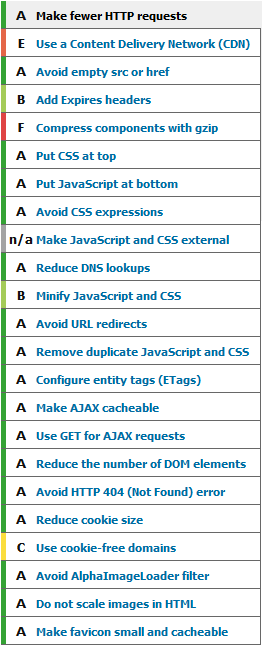
\includegraphics[keepaspectratio,scale=0.6]{images/nodeslow}}
	\subfigure[Yslow des Swift-Servers]{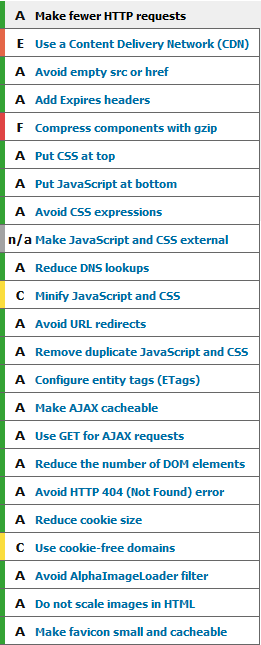
\includegraphics[keepaspectratio,scale=0.6]{images/swiftslow}}
\end{figure}

\subsection{Apache Bench}

Im ersten Schritt wird der Server mit 500 gleichzeitig durchgeführten Requests beauftrag bis insgesamt 5000 Requests abgehandelt wurden. Zur weiteren Überprüfung wird der Test mit 10.000, 20.000, 30.000, 40.000 und 50.000 zu je 500 parallelen Requests durchgeführt. Daraus wurde folgendes Ergebnis erstellt:

\begin{figure}[H]
\centering
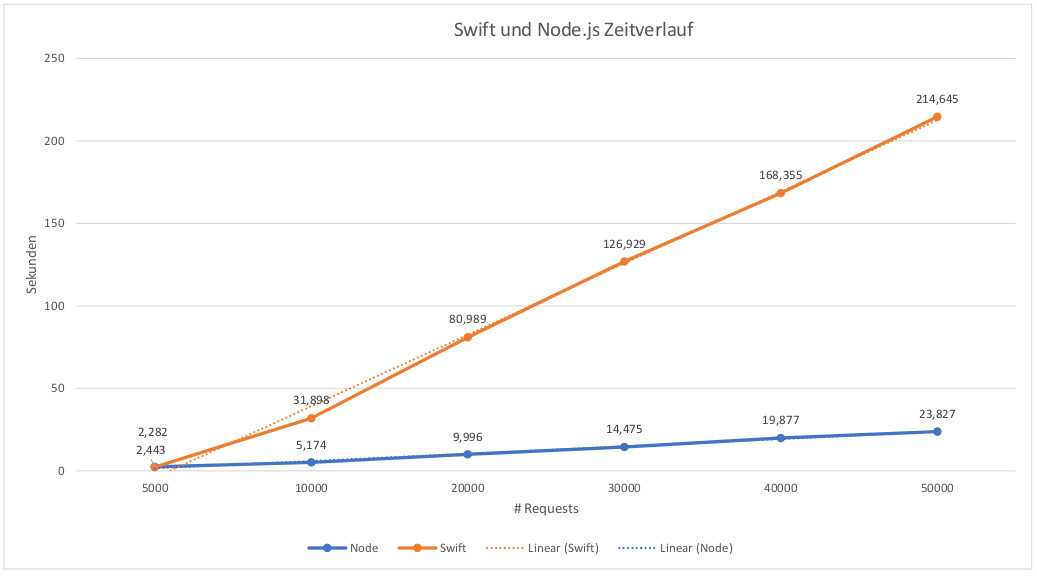
\includegraphics[keepaspectratio, scale = 0.4]{images/time.jpg}
\caption{Request-Abarbeitung von Express.js und Perfect}
\label{fig:time}
\end{figure}

\begin{table}[H]
\begin{center}
\begin{tabular}{p{8cm}p{2.5cm}p{2.5cm}}
\rowcolor{gray20}														& \textbf{Express.js}	  		& \textbf{Perfect}		\\ 
\rowcolor{gray5}		Document 											& LoginPage					& LoginPage			\\ 
\rowcolor{gray20}	Document Length										& 1.988 bytes				& 932 bytes			\\ 
\rowcolor{gray5}		Concurrency Level									& 500						& 500				\\ 
\rowcolor{gray20}	Time taken for tests [sec]								& 29,507					& 38,178			\\ 
\rowcolor{gray5}		Complete Requests									& 5.000						& 5.000				\\
\rowcolor{gray20}	Failed requests										& 0							& 0					\\ 
\rowcolor{gray5}		Total transferred [bytes]								& 11.070.000				& 6.950.000 			\\ 
\rowcolor{gray20}	HTML transferred	[bytes]								& 9.940.000					& 4.660.000			\\ 
\rowcolor{gray5}		Requests per second [\#/sec]							& 169,45					& 130,97			\\ 
\rowcolor{gray20}	Time per request [ms]	 (mean)							& 2.950,702					& 3.817,783			\\
\rowcolor{gray5}		Time per request [ms]	 (across concurrent requ.)			& 5,901						& 7,636				\\ 
\end{tabular}
\caption{Test: 5.000 Requests auf die "Login Page"} \label{tab:fivethousandrequests}
\end{center}
\end{table}

\begin{table}[H]
\begin{center}
\begin{tabular}{p{8cm}p{2.5cm}p{2.5cm}}
\rowcolor{gray20}														& \textbf{Express.js}	  		& \textbf{Perfect}		\\ 
\rowcolor{gray5}		Document 											& LoginPage					& LoginPage			\\ 
\rowcolor{gray20}	Document Length										& 1.988 bytes				& 932 bytes			\\ 
\rowcolor{gray5}		Concurrency Level									& 500						& 500				\\ 
\rowcolor{gray20}	Time taken for tests [sec]								& 172,275					& 273,546			\\ 
\rowcolor{gray5}		Complete Requests									& 50.000					& 50.000			\\
\rowcolor{gray20}	Failed requests										& 0							& 0					\\ 
\rowcolor{gray5}		Total transferred [bytes]								& 110.700.000				& 695.000.000		\\ 
\rowcolor{gray20}	HTML transferred	[bytes]								& 99.400.000				& 466.000.000		\\ 
\rowcolor{gray5}		Requests per second [\#/sec]							& 290,23					& 182,78			\\ 
\rowcolor{gray20}	Time per request [ms]	 (mean)							& 1.722,747					& 2735,462			\\
\rowcolor{gray5}		Time per request [ms]	 (across concurrent requ.)			& 3,445						& 5,471				\\ 
\end{tabular}
\caption{Test: 50.000 Requests auf die "Login Page"} \label{tab:fiftythousandrequests}
\end{center}
\end{table}

Bei dem Test wurde die Login-Page angefordert. Dabei änderte sich nur die Menge der Requests die abgehandlet werden mussten. Dadurch ergab es sich, dass die Menge der übertragenen Bytes linear anstgestiegen sind, die Zeit pro Request bei mehrmaligen durchlaufen jedoch stark schwankte. Die Differenz der Dokumentenlänge ergibt sich aus der unterschiedlich starken Kompression der Server. Somit blieb für die Abb. \ref{fig:time} nur ein Wert der sich auf beiden Seiten ändert, die \textit{Dauer des Tests}.

\section{Probleme und Lösungen}
Der Swift Server wurde auf einer VM getestet, die nur über eine CPU verfügt, wie bereits in \ref{sec:leistungsvergleich} erwähnt. Nachdem die VM um drei weitere Kerne auf 4 erweitert wurde, konnte der Server die Requests nicht mehr Ordnungsgemäß ausführen. Das lag daran, dass der Server nicht für Multitasking ausgelegt wurde, und der Server beim Bearbeiten von Requests versucht, gleichzeitig das benötigte HTML für mehrere Requests zusammenzubauen. Auf einem Rechner mit mehreren Kernen muss der Apache Bench insofern abgeändert werden, dass der \textit{Concurrency Level} auf 1 gestellt ist. Damit sind die Test jedoch wieder nicht aussagekräftig, und der Server müsste in diese Richtung überarbeitet werden. Schlussfolgernd, würde der Server auch ein viertel der Zeit benötigen, verglichen mit der derzeitigen Entwicklung.
Für die Testreihe müsste auch eine dezidierte und definierte Testumgebung festgelegt werden damit am nativen OS keine unterschiedlichen Prozesse die Ausführung der VirtualBox und damit die Test behindern bzw. beinflussen.

\chapterend

